\documentclass[paper=a4, fontsize=11pt]{scrartcl} % A4 paper and 11pt font size
\usepackage{./../usfassignment}
\usepackage{booktabs}
\settitle{Assignment 4}
\setauthor{Wanzhang Sheng}
\setcourse{CS662: Artificial Intelligent}

\begin{document}

\maketitle % Print the title

% -----------------------------------------------------------------------------
% PROBLEM 1
% -----------------------------------------------------------------------------
\section{}

\begin{fancyquotes}
  Write the following sentences in First-order logic

  \begin{enumerate}
    \item Any mortal holding the Ring will be tempted.
    \item Frodo is a hobbit.
    \item Hobbits are mortals.
    \item Anyone who is tempted will put on the Ring.
    \item If Frodo is not holding the ring, then Gandalf is holding it.
    \item Gandalf is not holding the Ring.
  \end{enumerate}

  You should use the following predicates: mortal(x), holding(x,y),
  tempted(x), hobbit(x), putOn(x,y).
\end{fancyquotes}

\begin{enumerate}
\item $\forall x$ \textit{mortal}($x$) $\land$
  \textit{holding}($x$,\textit{Ring}) $\Rightarrow$
  \textit{tempted}($x$)
\item \textit{hobbit}(\textit{Frodo})
\item $\forall x$ \textit{hobbit}($x$) $\Rightarrow$
  \textit{mortal}($x$)
\item $\forall x$ \textit{tempted}($x$) $\Rightarrow$
  \textit{putOn}($x$,\textit{Ring})
\item $\lnot$ \textit{holding}(\textit{Frodo}, \textit{Ring})
  $\Rightarrow$ \textit{holding}(\textit{Gandalf}, \textit{Ring})
\item $\lnot$ \textit{holding}(\textit{Gandalf}, \textit{Ring})
\end{enumerate}

%\pagebreak

% -----------------------------------------------------------------------------
% PROBLEM 2
% -----------------------------------------------------------------------------
\section{}

\begin{fancyquotes}
  Show that \textit{Frodo} has put on the \textit{Ring} using forward
  chaining. On each step, show the facts added to the KB and the list
  of substitutions.
\end{fancyquotes}

\begin{enumerate}
\item
((\textit{hobbit}(\textit{Frodo}))
$\land$
($\forall x$ \textit{hobbit}($x$) $\Rightarrow$ \textit{mortal}($x$))
$\implies$
(\textit{mortal}(\textit{Frodo}))
)\\
\{x/\textit{Frodo}\}

\item
(($\lnot$ \textit{holding}(\textit{Gandalf}, \textit{Ring}))
$\land$
($\lnot$ \textit{holding}(\textit{Frodo}, \textit{Ring}) $\Rightarrow$
\textit{holding}(\textit{Gandalf}, \textit{Ring})))
$\implies$
(\textit{holding}(\textit{Frodo}, \textit{Ring}))

\item
((\textit{mortal}(\textit{Frodo}))
$\land$
(\textit{holding}(\textit{Frodo}, \textit{Ring}))
$\land$
($\forall x$ \textit{mortal}($x$) $\land$
  \textit{holding}($x$,\textit{Ring}) $\Rightarrow$
  \textit{tempted}($x$)))
$\implies$
(\textit{tempted}(\textit{Frodo}))\\
\{x/\textit{Frodo}\}

\item
((\textit{tempted}(\textit{Frodo}))
$\land$
($\forall x$ \textit{tempted}($x$) $\Rightarrow$
\textit{putOn}($x$,\textit{Ring})))
$\implies$
(\textit{putOn}(\textit{Frodo}, \textit{Ring}))\\
\{x/\textit{Frodo}\}
\end{enumerate}

%\pagebreak

% -----------------------------------------------------------------------------
% PROBLEM 3
% -----------------------------------------------------------------------------
\section{}

\begin{fancyquotes}
  Show that \textit{Frodo} has put on the \textit{Ring} using backward
  chaining. Begin with \textit{putOn}(\textit{Frodo}, \textit{Ring})
  and work backward. At each step, show the queue of active goals.
\end{fancyquotes}

\begin{enumerate}
\item To prove:
  \begin{itemize}
  \item \textit{putOn}(\textit{Frodo}, \textit{Ring})
  \end{itemize}
\item To prove \textit{putOn}(\textit{Frodo}, \textit{Ring}), prove:
  \begin{itemize}
  \item \textit{tempted}(\textit{Frodo}) by 4
  \end{itemize}
\item To prove \textit{tempted}(\textit{Frodo}), prove:
  \begin{itemize}
  \item \textit{mortal}(\textit{Frodo}) by 1
  \item \textit{holding}(\textit{Frodo}, \textit{Ring}) by 1
  \end{itemize}
\item To prove \textit{mortal}(\textit{Frodo}), prove:
  \begin{itemize}
  \item \textit{hobbit}(\textit{Frodo}) by 3
  \item \textit{holding}(\textit{Frodo}, \textit{Ring})
  \end{itemize}
\item To prove \textit{holding}(\textit{Frodo}, \textit{Ring}), prove:
  \begin{itemize}
  \item \textit{hobbit}(\textit{Frodo})
  \item $\lnot$ \textit{holding}{\textit{Gandalf}, \textit{Ring}} by 5
  \end{itemize}
\item \textit{hobbit}(\textit{Frodo}) resolves with 2
\item $\lnot$ \textit{holding}{\textit{Gandalf}, \textit{Ring}}
  resolves with 6
\item Done.
\end{enumerate}

%\pagebreak

% -----------------------------------------------------------------------------
% PROBLEM 4
% -----------------------------------------------------------------------------
\section{}

\begin{fancyquotes}
  Use resolution with refutation to show that \textit{Frodo} has put
  on the \textit{Ring}. Show each step of the proof. You will first
  need to convert each of the sentences to CNF.

  Add $\lnot$ \textit{putOn}(\textit{Frodo}, \textit{Ring}) to the KB
  and derive a contradiction.
\end{fancyquotes}

\begin{enumerate}
\item $\lnot$ \textit{mortal}($x$) $\lor$ $\lnot$
  \textit{holding}($x$,\textit{Ring}) $\lor$ \textit{tempted}($x$)
\item \textit{hobbit}(\textit{Frodo})
\item $\lnot$ \textit{hobbit}($x$) $\lor$ \textit{mortal}($x$)
\item $\lnot$ \textit{tempted}($x$) $\lor$ \textit{putOn}($x$,\textit{Ring})
\item \textit{holding}(\textit{Frodo}, \textit{Ring}) $\lor$
  \textit{holding}(\textit{Gandalf}, \textit{Ring})
\item $\lnot$ \textit{holding}(\textit{Gandalf}, \textit{Ring})
\item $\lnot$ \textit{putOn}(\textit{Frodo}, \textit{Ring})
\item Resolve 4 and 7. Add $\lnot$ \textit{tempted}(\textit{Frodo})
\item Resolve 1 and 8. Add $\lnot$ \textit{mortal}(\textit{Frodo})
  $\lor$ $\lnot$ \textit{holding}(\textit{Frodo}, \textit{Ring})
\item Resolve 2 and 3. Add \textit{mortal}(\textit{Frodo})
\item Resolve 9 and 10. Add $\lnot$ \textit{holding}(\textit{Frodo},
  \textit{Ring})
\item Resolve 5 and 11. Add \textit{holding}(\textit{Gandalf},
  \textit{Ring})
\item Resolve 6 and 12. Contradiction!
\end{enumerate}

%\pagebreak

% -----------------------------------------------------------------------------
% PROBLEM 5
% -----------------------------------------------------------------------------
\section{}

\begin{fancyquotes}
  Work problem 13.8, parts a-d, from the R\&N textbook.
\end{fancyquotes}
\begin{table}[hp]
  \centering
  \begin{tabular}{ccccc}
    \toprule
    & \multicolumn{2}{c}{toothache} &
    \multicolumn{2}{c}{$\lnot$toothache}\\
    \midrule
    & catch & $\lnot$catch & catch & $\lnot$catch\\
    cavity & 0.108 & 0.012 & 0.072 & 0.008\\
    $\lnot$cavity & 0.016 & 0.064 & 0.144 & 0.576\\
    \bottomrule
  \end{tabular}
  \caption{A full joint distribution for the Toothache, Cavity, Catch world.}
\end{table}

\begin{enumerate}
\item P(toothache)\\
  = P(catch$\land$cavity) + P(catch$\land$$\lnot$cavity)
  + P($\lnot$catch$\land$cavity) + P($\lnot$catch$\land$$\lnot$cavity)\\
  = 0.108 + 0.016 + 0.012 + 0.064 = 0.2\\
\item P(cavity)\\
  = P(cavity$\land$toothache) + P(cavity$\land$$\lnot$toothache)\\
  = P(cavity$\land$catch$\land$toothache) +
  P(cavity$\land$catch$\land$$\lnot$toothache) +
  P(cavity$\land$$\lnot$catch$\land$toothache) +
  P(cavity$\land$$\lnot$catch$\land$$\lnot$toothache)\\
  = 0.108 + 0.012 + 0.072 + 0.008\\
  = 0.2
\item P(toothache$|$cavity)\\
  = P(toothache$\land$cavity) / P(cavity)\\
  = (P(catch$\land$cavity) + P($\lnot$catch$\land$cavity)) /
  P(cavity)\\
  = (0.108 + 0.012) / 0.2\\
  = 0.6
\item P(cavity$|$toothache$\lor$catch)\\
  = P(cavity$\land$(toothache$\lor$catch)) / P(toothache$\lor$catch)\\
  = (P(cavity$\land$toothache) + P(cavity$\land$catch)) /
  P(toothache$\lor$catch)\\
  = (0.108+0.012+0.072)/(0.108+0.012+0.072+0.016+0.064+0.144)\\
  = 0.461538462
\end{enumerate}


%\pagebreak

% -----------------------------------------------------------------------------
% PROBLEM 6
% -----------------------------------------------------------------------------
\section{}

\begin{fancyquotes}
  In the days before Canvas, Joe Student comes to his professor and
  tells her that he forgot to bring his project to hand in, and wants
  to turn it in tomorrow without penalty. The professor knows that 1
  time in 100, a student completes their assignment but forgets to
  bring it. The professor also knows that 50\% of the time, a student
  who hasn't completed the assignment will say that they forgot
  it. Finally, the professor believes that 90\% of the students in the
  class completed the assignment.

  What is the probability that the student actually completed the
  assignment?
\end{fancyquotes}
\begin{itemize}
\item P(completed$\land$forget) = 0.01
\item P(forget$|$$\lnot$completed) = 0.5
\item P(completed) = 0.9
\end{itemize}

P(completed$|$forget)\\
= P(completed$\land$forget) / P(forget)\\
= P(completed$\land$forget) / (P(forget$\land$completed) +
P(forget$\land$$\lnot$completed))\\
= P(completed$\land$forget) / (P(forget$\land$completed) +
P(forget$|$$\lnot$completed) * (1 - P(completed)))\\
= 0.01 / (0.01 + 0.5 * (1 - 0.9))\\
= 0.166666667

%\pagebreak

% -----------------------------------------------------------------------------
% PROBLEM 7
% -----------------------------------------------------------------------------
\section{}

\begin{fancyquotes}
  Work problem 23.3, parts a-d, from the R\&N textbook. Part C is
  asking about ambiguity as discussed on p.905.
\end{fancyquotes}

\begin{enumerate}
\item ``shoots the duck well well well'' has nonzero probability.
\item Probability of generating ``is well well'' is
  $0.2^{2}\times 0.1\times 0.5^{3} + 0.2^{2}\times 0.8\times 0.5^{2}
  = 0.0005 + 0.008 = 0.0085$.
\item Ambiguity type of (b) is
  syntactic ambiguity since there is two parse tree for this sentence.
  %lexical ambiguity since ``well'' has more than one meaning.
\item
  It's possible to calculate the probability the string of exactly
  10 words generated by the given PCFG.
  Because we can simply enumerate all strings of exactly 10 words.
  And stop further search when we already have 10 symbols to avoid
  infinity loop, since symbols will end in at least one terminal
  words.
\end{enumerate}
%\pagebreak

% -----------------------------------------------------------------------------
% PROBLEM 8
% -----------------------------------------------------------------------------
\section{}

\begin{fancyquotes}
  Work problem 23.6 from the R\&N textbook; be sure to read and answer
  the entire question up to the start of problem 23.7.
\end{fancyquotes}

\begin{figure}[hp]
  \centering
  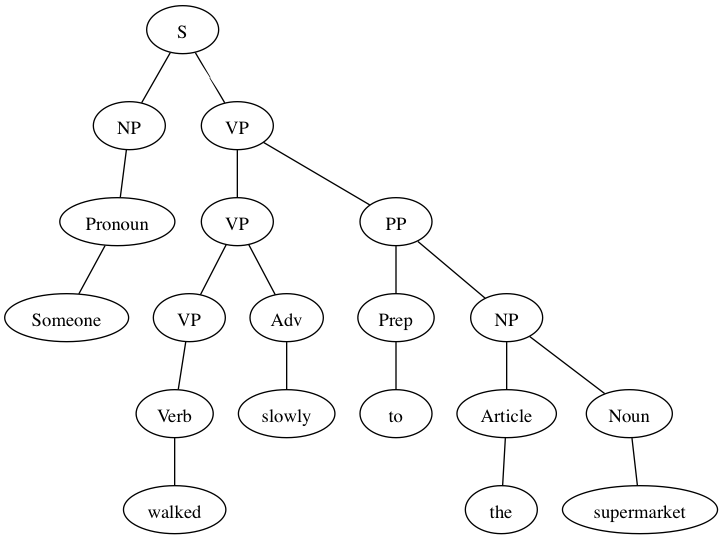
\includegraphics[width=.7\textwidth]{4-8.gv.png}
  \caption{A grammer}
\end{figure}

\begin{figure}[hp]
  \centering
  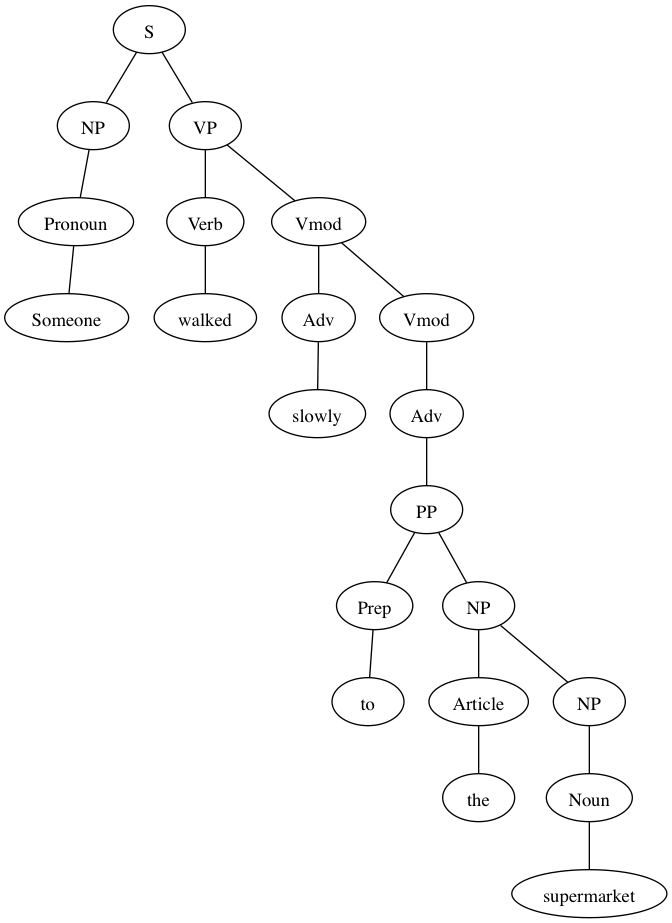
\includegraphics[width=.7\textwidth]{4-8.gv.2.png}
  \caption{B grammer}
\end{figure}

\begin{figure}[hp]
  \centering
  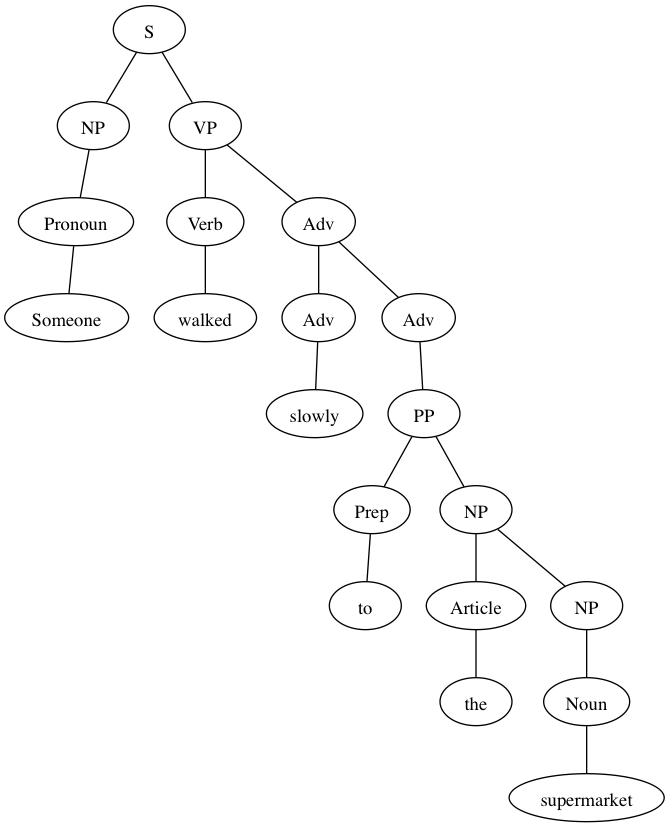
\includegraphics[width=.7\textwidth]{4-8.gv.3.png}
  \caption{C grammer}
\end{figure}

\subsection{A}

\begin{itemize}
\item Article $\rightarrow$ a
\item Noun $\rightarrow$ apple
\item Prep $\rightarrow$ at
\item Noun $\rightarrow$ bananas
\item Verb $\rightarrow$ beat
\item Verb $\rightarrow$ eat
\item Verb $\rightarrow$ fall
\item Adv $\rightarrow$ fastly
\item Noun $\rightarrow$ ground
\item Pronoun $\rightarrow$ i
\item Prep $\rightarrow$ in
\item Noun $\rightarrow$ jack
\item Verb $\rightarrow$ like
\item Adv $\rightarrow$ loudly
\item Pronoun $\rightarrow$ me
\item Noun $\rightarrow$ monkey
\item Noun $\rightarrow$ school
\item Verb $\rightarrow$ sing
\item Adv $\rightarrow$ slowly
\item Noun $\rightarrow$ time
\item Pronoun $\rightarrow$ tom
\item Adv $\rightarrow$ very
\item Adv $\rightarrow$ well
\item Noun $\rightarrow$ yard
\item Pronoun $\rightarrow$ you
\item Noun $\rightarrow$ zoo
\end{itemize}

English:
\begin{enumerate}
\item The apple falls to the ground at the time.
\item Tom sings loudly in the yard.
\item Monkeys like the bananas very well in the zoo.
\end{enumerate}

Non-English:
\begin{enumerate}
\item I eat well well well well well well.
\item A Jack eat to a Jack fastly slowly.
\item Me beat you in the school.
\end{enumerate}

Remove:\\
VP $\rightarrow$ VP adv\\
Replace:\\
VP $\rightarrow$ Verb\\
by:\\
VP $\rightarrow$ Verb Adv

\subsection{B}

English:
\begin{enumerate}
\item I love the Apple very well.
\item The apple falls very very slowly.
\item I beat the monkey very fastly.
\end{enumerate}

Non-English:
\begin{enumerate}
\item The the the the apple eat slowly.
\item Apple eat well well well well well the apple.
\item I eat the monkey the monkey.
\end{enumerate}

Replace:\\
NP $\rightarrow$ Article NP\\
by:\\
NP $\rightarrow$ Article Noun\\
NP $\rightarrow$ Article Pronoun

\subsection{C}

English:
\begin{enumerate}
\item I beat the monkey very slowly.
\item Jack sing slowly to the monkey.
\item Tom like Jack very very well.
\end{enumerate}

Non-English:
\begin{enumerate}
\item A a a a a Tom fall slowly.
\item Monkey fall fastly slowly fastly slowly.
\item Me beat to apple to jack.
\end{enumerate}

Replace:\\
NP $\rightarrow$ Article NP\\
by:\\
NP $\rightarrow$ Article Noun\\
NP $\rightarrow$ Article Pronoun


Ultimate method to fix the grammer is to use non-Context-Free Grammer,
such as Unstricted-Grammer.
Since English is not a context free language, it can't be expressed
well in context free grammer.

%\pagebreak

\end{document}
